\section{Github Fork Maintenance}\label{s:github-fork-maintenance}

\subsection{Introduction to Github}
Github Fork maintenance is a very important thing when you are
developiing applications in groups. Github acts as a source which
keeps the versions of the files that we submit in the Github depending
on our commits. In Github commits means you are creating, deleting or
updating a content in the Github reporitory.

\subsection{Fork a Repository}

First go to the following repository using youre preferred web
browswer.

\href{https://www.github.com/cloudmesh/book}{Cloudmesh Repository}

\begin{figure}[htb]\label{fig:howtofork}
\centering
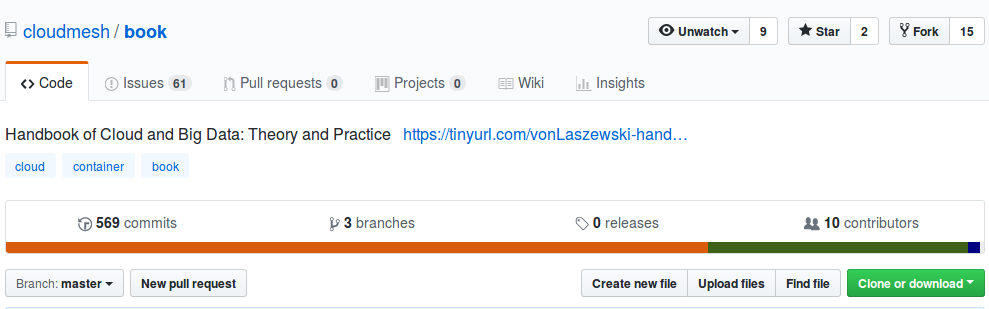
\includegraphics[width=1.0\textwidth]{fork-howtofork.png}
\caption{Forking Cloudmesh Book Repository
}
\end{figure}

Referring to Figure \ref{fig:howtofork}, click the fork button on the
top right of your browser window. After clicking this button, you will
have to select your profile in the pop up window and fork it. Then it
will generate your fork. Basically a fork represents your own copy of
an existing repository. If you have dond everything successfully, you
can see the results as in Figure \ref{fig:myfork}.

\begin{figure}[htb]\label{fig:myfork}
\centering
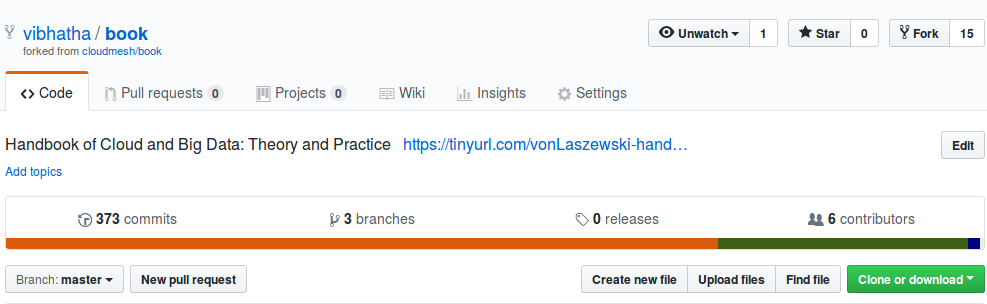
\includegraphics[width=1.0\textwidth]{fork-lookslike.png}
\caption{Successful Fork Output
}
\end{figure}

\subsection{Clone a Fork}

Now you have to clone the fork you have created in to your machine.
Refer to the Figure \ref{fig:clonemyfork} and copy the fork link
first by clicking clone or download button and copy the fork link.

\begin{NOTE}
  Selecte Use SSH setting and make sure you have used uploaded a
  SSH key to Github before doing this. Follow the chapter \ref{C:ssh} if you have not already generated SSH for Github.
\end{NOTE}


\begin{figure}[htb]\label{fig:clonemyfork}
\centering
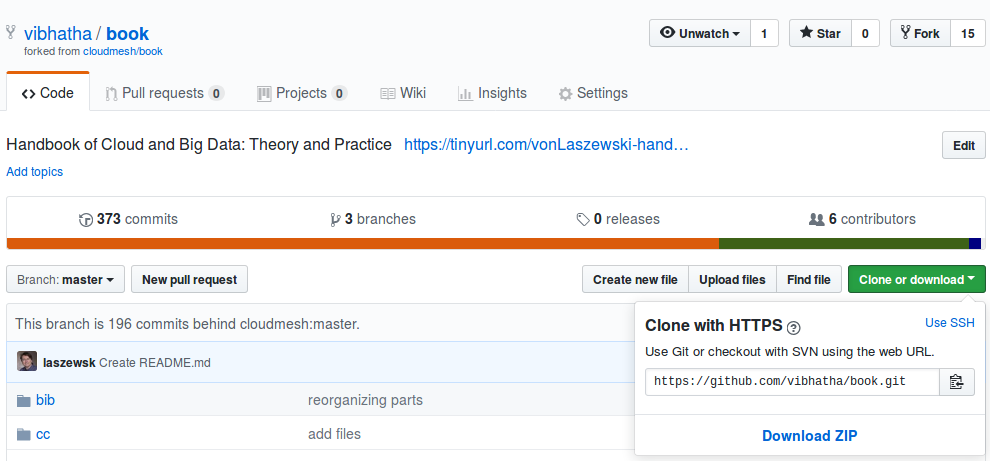
\includegraphics[width=1.0\textwidth]{fork-clonefork.png}
\caption{Clonning a Fork
}
\end{figure}

Next go to the terminal and do the execute the following commands

\begin{NOTE}
 In the commands replace <github-username> with your Github username
\end{NOTE}

\begin{lstlisting}
mkdir -p ~/cloudmesh/fork
cd ~/cloudmesh/fork
git clone https://github.com/<github-username>/book.git  
\end{lstlisting}

If no errors pop up, you have successfully cloned your fork.

\subsection{Set Up Upstream}

Run the following commands in your terminal window.

\begin{lstlisting}
cd ~/cloudmesh/fork/book
git remote -v
\end{lstlisting}

After running the last command you will see the following
output.

\begin{lstlisting}
origin	git@github.com:<github-username>/book.git (fetch)
origin	git@github.com:<github-username>/book.git (push) 
\end{lstlisting}

Here you have to set up the upstream now. By default the upstream is
not set.

The syntax for setting upstream as follows,

\begin{lstlisting}
git remote add upstream https://github.com/ORIGINAL_OWNER/ORIGINAL_REPOSITORY.git
\end{lstlisting}

For our project, it looks the following.
Run the following command in your terminal.

\begin{lstlisting}
git remote add upstream https://github.com/cloudmesh/book.git
\end{lstlisting}

Now do the following to make sure you have successfully set up the upstream.

\begin{lstlisting}
git remote -v  
\end{lstlisting}

\begin{NOTE}
 Instead of <github-username>, you will see your username. 
\end{NOTE}

\begin{lstlisting}
origin	git@github.com:<github-username>/book.git (fetch)
origin	git@github.com:<github-username>/book.git (push)
upstream	https://github.com/cloudmesh/book.git (fetch)
upstream	https://github.com/cloudmesh/book.git (push)
\end{lstlisting}

If you see the above output, you have successfully set up the upstream.

\subsection{Fetch Upstream}

In practical sense, your fork is your own copy of the original
repository.  But at some point, you need to keep yourself updated with
the original fork.  In this step, you may need to fetch records from
the upstream or the original repository. In this case first run the
following command to fetch newly added commits for your local file
system. This doesn't sync your fork with the original repository. For this
tutorial we assume everyone is going to work in the master branch.

Run the following command inside the forked branch in your local machine

\begin{lstlisting}
  cd ~/cloudmesh/fork/book
  git fetch upstream
\end{lstlisting}

Generally if there are no new updates after the time you fork the main
repository, you will see something like this in the terminal as the
output.

\begin{lstlisting}
remote: Counting objects: 1648, done.
remote: Compressing objects: 100% (42/42), done.
remote: Total 1648 (delta 758), reused 777 (delta 746), pack-reused 857
Receiving objects: 100% (1648/1648), 9.80 MiB | 2.56 MiB/s, done.
Resolving deltas: 100% (1191/1191), completed with 162 local objects.
From https://github.com/cloudmesh/book
 * [new branch]      dev        -> upstream/dev
 * [new branch]      latex      -> upstream/latex
 * [new branch]      master     -> upstream/master
\end{lstlisting}

This command fetches the branches and their respective commits from
the upstream repository that we set up earlier. Now select a
particular bracnh.  Here we select the master branch.

Run the following command to select the master branch.

\begin{lstlisting}
  git checkout master
\end{lstlisting}

\subsection{Merge With Upstream}

Now what you have to do is you have to merge the changes you took from
the upstream to your local master branch. By doing this, your fork's
master branch will be in sync with the upstream along with local
changes being updated there. For that run the following commands in
your terminal.

Before doing this you can change your files in the local machine
implying the files related to your fork. In practical case you do
merging once you have successfully completed a particular task and
then you will merge that with the master branch in the original
repository. This is the way collaboration works.

\begin{lstlisting}
  git merge upstream/master
\end{lstlisting}

If there are no conflicts, this will successfully merge with the master. 
If you don't have any changes in the local branch (unique commits), git
will do a fast-forward.

The following shows a sample fast-forward action. 
\begin{lstlisting}
  Updating d8676c9..e6cc9cf
Fast-forward
 .travis.yml                                                      |   50 ++
 Makefile                                                         |   65 ++-
 bib/bibliography.bib                                             |    0
 bib/refs-mqtt.bib                                                |  310 ++++++++++++
 bin/md-all-to-tex.py                                             |   18 +
 bin/md-image-fetch.py                                            |   87 ++++
 bin/md-to-tex.py                                                 |   65 +++
 cloud.tex                                                        |    0
 deprecated/chapter-latex/lesson/doc/latex.tex                    |   40 +-
 {section/iot => deprecated}/dexter.md                            |    0
 {section/iot => deprecated}/esp8266.md                           |    0
 {section => deprecated}/eve.tex                                  |   14 +-
...
\end{lstlisting}

\subsection{Pull Requests}

Pull requests is also an interestig topic when we work with
forks. Once you have an already synced fork with the original
repository, you will need to commit the changes to your fork. Then you
will just use basic commiting method, first you add a file using git
add and push the changes with git push. Here is an example.

Let's assume you change a file called readme.md,

\begin{lstlisting}
  git add readme.md
  git commit -m ``updated readme'' readme.md
  git push origin master
\end{lstlisting}

Here you will push the commits to the origin in master. The origin is
your fork. So how will the original repository know about your changes.
Here you need to make a pull request to the original branch. 

Once you have a latest commit to your fork, when you go to the web
browswer and navigate to your fork, you will see that there is an
update and your fork is ahead of one commit with reference to the
original repository.

\begin{figure}[htb]\label{fig:forkcommit}
\centering
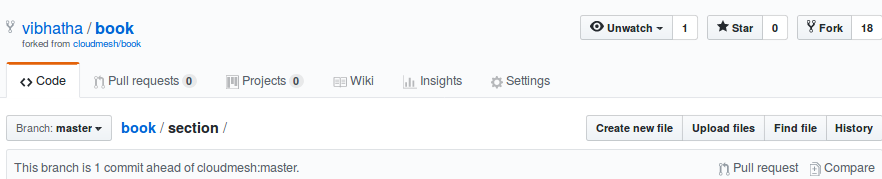
\includegraphics[width=1.0\textwidth]{fork-gitcomit.png}
\caption{Fork Gets a New Commit
}
\end{figure}

It will say something like shown in the figure \ref{fig:forkcommit},
saying this branch is ahead of cloudmesh master.

Now you need to tell the cloudmesh master that you need to get updates
from your fork. This is the pull request concept.


\begin{figure}[htb]\label{fig:forkpullrequest}
\centering
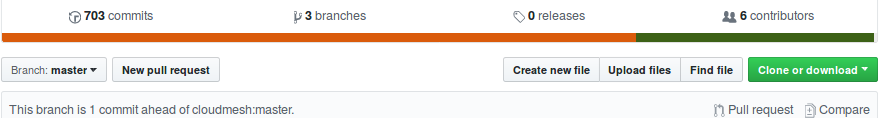
\includegraphics[width=1.0\textwidth]{fork-pullrequest.png}
\caption{Create a New Pull Request
}
\end{figure}

Referring to figure \ref{fig:forkpullrequest}, create a new pull
request. If you have successfully created a pull request and if it
doesn't have any conflicts it will say that it is possible to merge as
well.  Figure \ref{fig:forkpullrequestinfo} will show the response.


\begin{figure}[htb]\label{fig:forkpullrequestinfo}
\centering
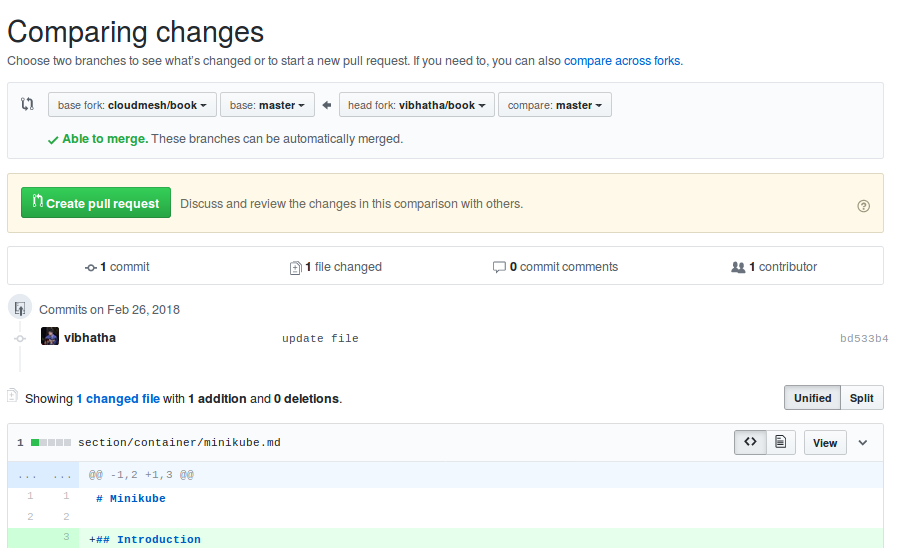
\includegraphics[width=1.0\textwidth]{fork-pullrequestcrt.png}
\caption{Pull Request Response
}
\end{figure}

Here you have to creat the pull request by clicking the Create Pull
Request button in the GUI in the web interface popping up. After
clciking that you will have to create the pull request with a clear
detail explaining what you did as shown in figure
\ref{fig:forkpullrequestcr}.


\begin{figure}[htb]\label{fig:forkpullrequestcr}
\centering
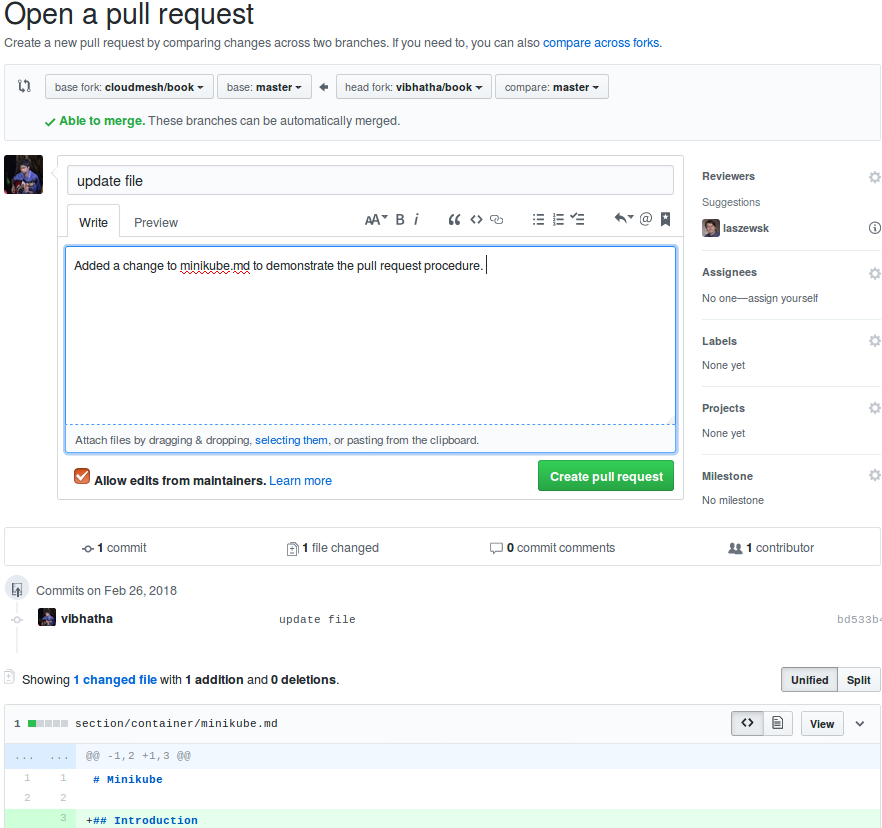
\includegraphics[width=1.0\textwidth]{fork-createpullrq.png}
\caption{Pull Request Response
}
\end{figure}

Click the create pull request button to finalize your pull request. 

Here you have successfully created a pull request. It will be shown
in the Original repository as shown in figure \ref{fig:pullreqincm}.

\begin{figure}[htb]\label{fig:pullreqincm}
\centering
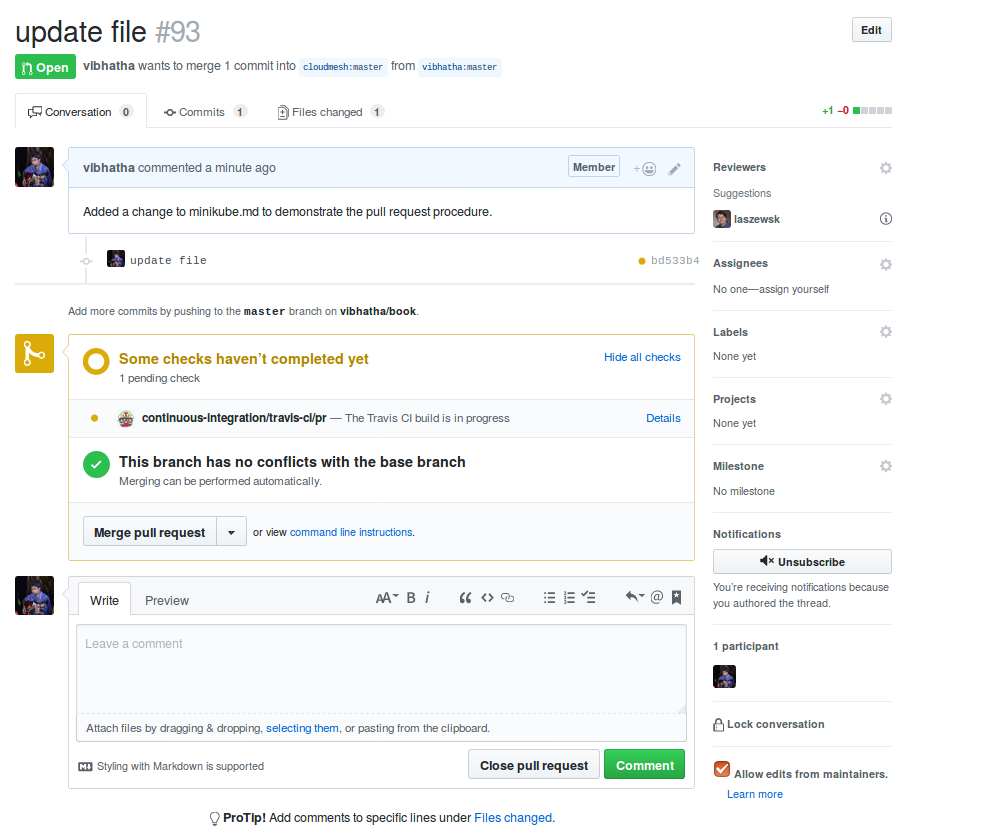
\includegraphics[width=1.0\textwidth]{fork-pullrequestcm.png}
\caption{Pull Request Shown In original Repository. 
}
\end{figure}

Here it will show that Travis is till working on it. And finally if
there are no conflicts it will show that it can be merged. But it is a
duty of someone else or you. But here we recommend not to accept your
own pull requests. Assign it to one of the TAs or Professor to acccept
the pull request.

This section explains you how to keep your fork in sync with original
repository and make pull requests to notify your work. 
